%
% Complete documentation on the extended LaTeX markup used for Insight
% documentation is available in ``Documenting Insight'', which is part
% of the standard documentation for Insight.  It may be found online
% at:
%
%     http://www.itk.org/

\documentclass{InsightArticle}

\usepackage[dvips]{graphicx}


% Personal settings for code snippets visualization
% For code snippets style definition

\usepackage{color}
\usepackage{listings}


\lstloadlanguages{[ISO]C++,C}
% set up listing environment with C syntax hightlight
\definecolor{stringcolor}{rgb}{0.20,0.50,0.20}
\definecolor{commentcolor}{rgb}{0.40,0.40,0.40}
\definecolor{keywordcolor}{rgb}{0.50,0.10,0.10}
\definecolor{idcolor}{rgb}{0.10,0.10,0.50}
\definecolor{bg}{rgb}{0.95,0.95,0.95}
% with \lstset one can predefine parameters for listings
%\lstset{language=[ISO]C++,basicstyle=\small,keywordstyle=\color{keywordcolor},
 %       commentstyle={\color{commentcolor}\itshape},
%        stringstyle={\color{stringcolor}},
%        identifierstyle=\color{idcolor},numbers=left,
       % xleftmargin=2em,framerule=0.8pt,
%        stepnumber=1,frame=single,showstringspaces=false,
%        firstnumber=1,numberstyle=\ttfamily,backgroundcolor=\color{bg}}
 
\lstset{ %
  language=[ISO]C++,                % choose the language of the code
  basicstyle={\small\ttfamily},       % the size of the fonts that are used for the code
  keywordstyle=\color{keywordcolor},
  stringstyle={\color{stringcolor}},
  identifierstyle=\color{idcolor},
  numbers=left,                   % where to put the line-numbers
  numberstyle=\footnotesize,      % the size of the fonts that are used for the line-numbers
  stepnumber=1,                   % the step between two line-numbers. If it's 1 each line 
                                % will be numbered
  numbersep=5pt,                  % how far the line-numbers are from the code
  backgroundcolor=\color{white},  % choose the background color. You must add \usepackage{color}
  showspaces=false,               % show spaces adding particular underscores
  showstringspaces=false,         % underline spaces within strings
  showtabs=false,                 % show tabs within strings adding particular underscores
  frame=single,	                % adds a frame around the code
  tabsize=2,	                % sets default tabsize to 2 spaces
  captionpos=t,                   % sets the caption-position to bottom
  breaklines=true,                % sets automatic line breaking
  breakatwhitespace=false,        % sets if automatic breaks should only happen at whitespace
  title=\lstname,                 % show the filename of files included with \lstinputlisting;
                                % also try caption instead of title
  escapeinside={\%*}{*)},         % if you want to add a comment within your code
  }
 
% rotate images 
\usepackage{rotating}
        
% Definition of \C++ to be eye candy :
\usepackage{relsize}
\usepackage{lipsum}
%c from texinfo.tex
\def\ifmonospace{\ifdim\fontdimen3\font=0pt }
\def\C++{%
\ifmonospace%
    C++%
\else%
    C\kern-.1667em\raise.30ex\hbox{\smaller{++}}%
\fi%
\spacefactor1000 }


%%%%%%%%%%%%%%%%%%%%%%%%%%%%%%%%%%%%%%%%%%%%%%%%%%%%%%%%%%%%%%%%%%
%
%  hyperref should be the last package to be loaded.
%
%%%%%%%%%%%%%%%%%%%%%%%%%%%%%%%%%%%%%%%%%%%%%%%%%%%%%%%%%%%%%%%%%%
\usepackage[dvips,
bookmarks,
bookmarksopen,
backref,
colorlinks,linkcolor={blue},citecolor={blue},urlcolor={blue},
]{hyperref}


%  This is a template for Papers to the Insight Journal. 
%  It is comparable to a technical report format.

% The title should be descriptive enough for people to be able to find
% the relevant document. 
\title{A simple Qt based comparison program\\ for ITK and VTK images.}

% 
% NOTE: This is the last number of the "handle" URL that 
% The Insight Journal assigns to your paper as part of the
% submission process. Please replace the number "1338" with
% the actual handle number that you get assigned.
%
\newcommand{\IJhandlerIDnumber}{3196}

% Increment the release number whenever significant changes are made.
% The author and/or editor can define 'significant' however they like.
\release{0.00}

% At minimum, give your name and an email address.  You can include a
% snail-mail address if you like.
\author{Antonin Perrot-Audet, Arnaud Gelas, Kishore Mosaliganti,\\ 
Nicolas Rannou, Lydie Souhait, Sean Megason}
\authoraddress{ Harvard Medical School, Megason lab}
            %   $^{1}$Harvard Medical School, Megason lab\\
            %   $^{2}$Rome University, Inquisition street\\
            %   $^{3}$Netherlands Pragmatic University, Port street

\begin{document}

% Add hyperlink to the web location and license of the paper.
\IJhandlefooter{\IJhandlerIDnumber}


\ifpdf
\else
   %
   % Commands for including Graphics when using latex
   % 
   \DeclareGraphicsExtensions{.eps,.jpg,.gif,.tiff,.bmp,.png}
   \DeclareGraphicsRule{.jpg}{eps}{.jpg.bb}{`convert #1 eps:-}
   \DeclareGraphicsRule{.gif}{eps}{.gif.bb}{`convert #1 eps:-}
   \DeclareGraphicsRule{.tiff}{eps}{.tiff.bb}{`convert #1 eps:-}
   \DeclareGraphicsRule{.bmp}{eps}{.bmp.bb}{`convert #1 eps:-}
   \DeclareGraphicsRule{.png}{eps}{.png.bb}{`convert #1 eps:-}
\fi

\maketitle

\ifhtml
\chapter*{Front Matter\label{front}}
\fi

\begin{abstract}
\noindent
This document describes a project that can compare many images simultaneously in a synchronized manner. Such an application can be used in any ITK/VTK image processing pipelines; the programmer can use it to quickly visualize and compare intermediate results of used filters within the pipeline.The goals of this project are two folds: (i) to be integrated in gdb pretty debuggers \cite{McCornic-VisualDebug}  (for visual debugging of ITK pipelines), and, (ii) to provide a visual comparison widget for image-to-image plugins (ITK or VTK based filters).\\
This project is part of the Gofigure2 \cite{refGofigure2} development effort, an open-source, cross-platform application for visualizing, processing and analyzing of multidimensional microscopy data. 
\end{abstract}

\IJhandlenote{\IJhandlerIDnumber}

\tableofcontents

Based on Qt libraries \cite{refQT}, ITK \cite{ITKSoftwareGuide}, VTK \cite{vtkExamples}, and MegaVTK (a variant of vtkINRIA3D engine \cite{vtkINRIA}), we developed an application for multiple image visualization and comparison.
We provide the following items in this submission:
\begin{itemize}
 \item a set of classes and widgets for simple integration in a generic program developed by a user,
 \item an executable for command line usage (compareexample).
\end{itemize} 

\section{Principle}
In order to make these classes easy to use and modify, we created an instance of \code{QWidget} using a form (.ui file) for the GUI using Qt Designer. We also created a manager class that takes care of widgets creation, deletion and synchronization. The manager class (\code{QObject}) automatically takes care of the following issues:
\begin{itemize}
  \item Support for ITK images
  \item Support for VTK images
  \item Camera synchronization for fine comparison of results.
  \item QWidget inheritance for integration to an external application with Qt-based GUI.
%  \item doxygen documentation
\end{itemize}


\section{Examples and Documentation}
\subsection*{Documentation}
The library is composed of six classes :
\begin{description}
  \item [\href {http://gofigure2.sourceforge.net/Doxygen/Nightly/html/classQGoSynchronizedView.html}{QGoSynchronizedView}]
    abstract class for QGoSynchronizedView2D and QGoSynchronizedView3D.
    
  \item [\href {http://gofigure2.sourceforge.net/Doxygen/Nightly/html/classQGoSynchronizedView2D.html}{QGoSynchronizedView2D}]
    class is used to display a QWidget containing a two dimensional vtkimagedata* or itkimage*. QGoSynchronizedView2D provides the interface to synchronize cameras among several GoSynchronizedView2D objects.
    
  \item [\href {http://gofigure2.sourceforge.net/Doxygen/Nightly/html/classQGoSynchronizedView2DCallbacks.html}{QGoSynchronizedView2DCallbacks}]
    This object takes a list of QGoSynchronizedView objects and synchronizes their cameras by setting up appropriate callbacks. It is recommended to let the QGoSynchronizedViewManager deal with synchronization of objects since it simplifies the burden on the user significantly.
    
  \item [\href {http://gofigure2.sourceforge.net/Doxygen/Nightly/html/classQGoSynchronizedView3D.html}{QGoSynchronizedView3D}]class is used to display a QWidget containing a three dimensional vtkimagedata* or itkimage*. QGoSynchronizedView3D provides the interface to synchronize cameras among several GoSynchronizedView3D obhects.
  
  \item [\href {http://gofigure2.sourceforge.net/Doxygen/Nightly/html/classQGoSynchronizedView3DCallbacks.html}{QGoSynchronizedView3DCallbacks}]
    This object takes a list of QGoSynchronizedView objects and synchronizes their cameras by setting up appropriate callbacks. It is recommended to let the QGoSynchronizedViewManager deal with synchronization of objects since it simplifies the burden on the user significantly.
  
  \item [\href {http://gofigure2.sourceforge.net/Doxygen/Nightly/html/classQGoSynchronizedViewManager.html}{QGoSynchronizedViewManager}]
  High level class for QGoSynchronizedView2D, QGoSynchronizedView2DCallbacks, QGoSynchronizedView3D, QGoSynchronizedView3DCallbacks. This class deals with QGoSynchronizedViews for correct synchronization and provides a simple interface to create/delete/synchronize QGoSynchronizedViews. This class should be used with any class using QGoSynchronizedView and QGoSynchronize.
  
\end{description}

For implementation details, the reader is directed to the \href {http://gofigure2.sourceforge.net/Doxygen/Nightly/} {Doxygen documentation} and the source code which is extensively documented.

\subsection*{Code Snippets}
We introduce here the high level functions for creating QWidgets views and synchronizing visualizations:
\large
  \begin{lstlisting}[title={\large Creation of the visualization manager object}]{high_level_creation_visu_manager}
/* we simply create a new manager that will take care of 
 * creation/deletion of visualization and callbacks for us.
 */
QGoSynchronizedViewManager* ViewManager = new QGoSynchronizedViewManager();

// Visualize some images, process etc...

// Remember to delete ViewManager when no visualization is needed
delete ViewManager;
  \end{lstlisting}
\normalsize
\large
  \begin{lstlisting}[title={\large Visualization of a VTK image}]{high_level_creation_visu_VTK}
/*  the synchronization manager can create visualization windows given
 *  a valid pointer to a VTK image and 
 *  a string encoding the name of the visualization.
 */
ViewManager->newSynchronizedView("My VTK View", VTKSmartPointerToImage);
ViewManager->Update();
ViewManager->show();
  \end{lstlisting}
\normalsize
\large
  \begin{lstlisting}[title={\large Visualization of an ITK image}]{high_level_creation_visu_ITK}
/*  the synchronization manager can create visualization windows given
 *  a valid pointer to an ITK image,
 *  the template argument representing the image pixel type,
 *  a string encoding the name of the visualization.
 */
ViewManager->newSynchronizedView<InputPixelType>
  ("My ITK View", ITKSmartPointerToImage);
ViewManager->Update();
ViewManager->show();
  \end{lstlisting}
\normalsize
\large
  \begin{lstlisting}[title={\large Synchronization of the camera for several images}]{high_level_synchro_visu}
/*  the synchronization manager can synchronize the opened images 
 *  with a simple function call
 */
ViewManager->synchronizeOpenSynchronizedViews();
  \end{lstlisting}
\normalsize

\subsection*{Code Examples}
The code source is delivered with several tests and examples, located in Examples/GUI/lib/
Three examples illustrate the code snippets introduced in this article :
\begin{description}
  \item [compareexample] takes a list of 2D or 3D images as an input and displays them in synchronized viewer widgets.
  \item [comparepipelineexample] takes a 2D or 3D image as an argument and displays this images before and after filtering by a Gaussian filter. 
  \item [compareguiexample] shows how to create a very basic GUI using the functionalities provided by the \code{QGoSynchronized} classes. Figure ~\ref{fig:ImageCompareGUIquad} and ~\ref{fig:ImageCompareGUIXY} are screenshots of this application.
\end{description}


\section{Installation}
\subsection*{Software Requirements}
You need to have the following software installed:
\begin{itemize}
  \item  Insight Toolkit 3.18 (or higher)
  \item  Visualization Toolkit 5.6.0 (or higher)
  \item  CMake 2.4 (or higher)
\end{itemize}

\subsection*{Compiling from sources on Linux/MacOsX}
Get the latest version of the program from the GIT repository :
\begin{lstlisting}[language=ksh,numbers=none,captionpos=none]
$ git clone git://github.com/antonin07130/itkCompareProject.git 
$ cd itkCompareProject
\end{lstlisting}
Create a build directory where the compare examples will be compiled
\begin{lstlisting}[language=ksh,numbers=none,captionpos=none]
$ mkdir BUILD
\end{lstlisting}
Launch cmake
\begin{lstlisting}[language=ksh,numbers=none,captionpos=none]
$ cd BUILD
$ ccmake path/to/source/directory
\end{lstlisting}
Build
\begin{lstlisting}[language=ksh,numbers=none,captionpos=none]
$ make
\end{lstlisting}
Test
\begin{lstlisting}[language=ksh,numbers=none,captionpos=none]
$ ctest
\end{lstlisting}
The binaries are located in BUILD/bin/ 

\section{Future work}
In the future, we plan to :
\begin{itemize}
  \item Integrate this application into gdb pretty debugger for ITK.
  \item Add more pixel types for itk images (vector, tensor images),
  \item Add more features (generate the difference of two images, overlays...)
\end{itemize}

\begin{figure}[p]
\center
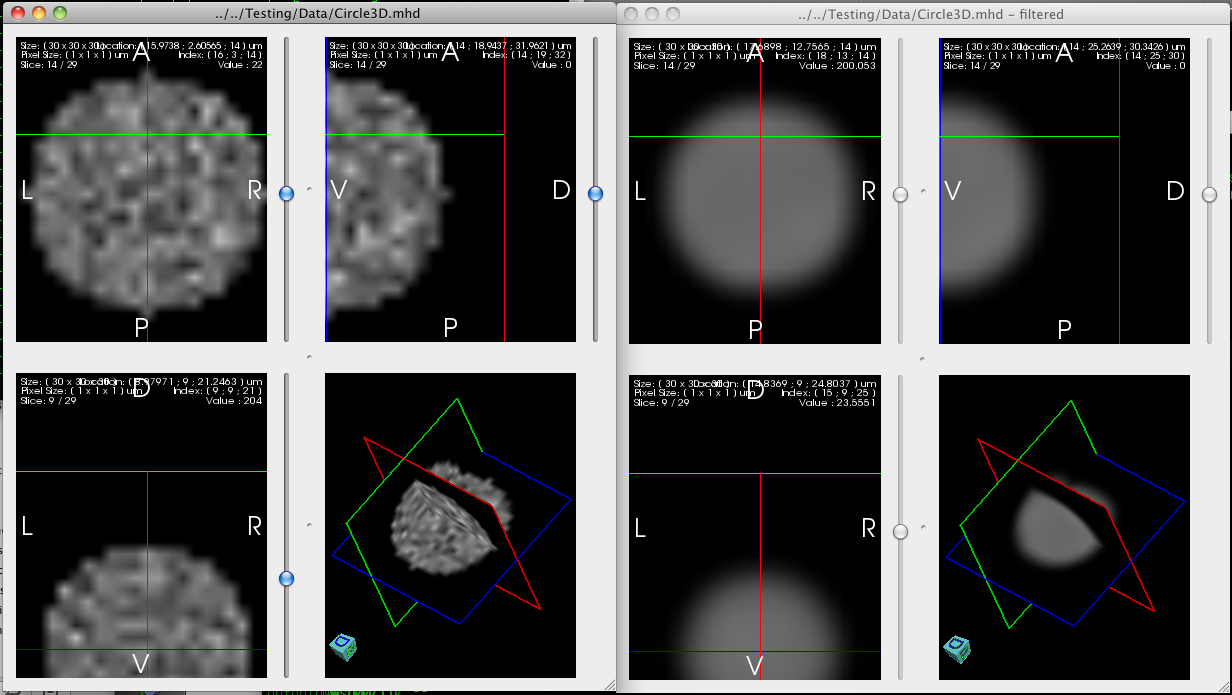
\includegraphics[width=1\textwidth]{images/quadcompare}
\itkcaption[Pipeline Input/Output comparison]{"./compareguiexample" on MacOsX 10.6. The user compares two 3D data sets and uses the quadview to compare them. The quadview provides three the orthogonal views and one isometric 3D view.}
\label{fig:ImageCompareGUIquad}
\end{figure}

\begin{figure}[p]
\center
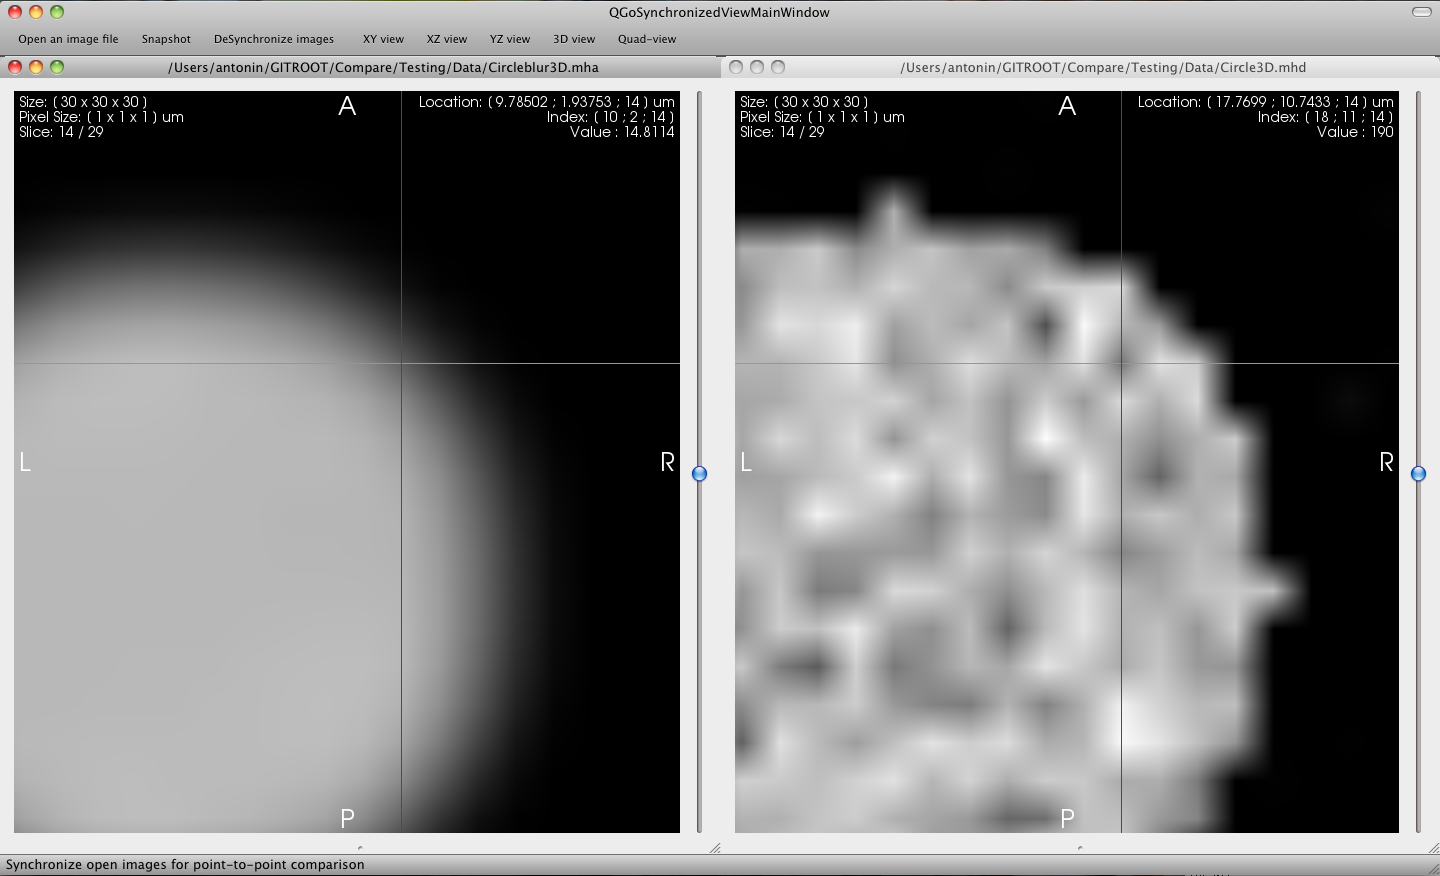
\includegraphics[width=1\textwidth]{images/xycompare}
\itkcaption[Pipeline Input/Output comparison]{"./compareguiexample" on MacOsX 10.6. The user compares two 3D data sets by visualizing the XY view specifically.}
\label{fig:ImageCompareGUIXY}
\end{figure}

%figures :
\clearpage

\bibliographystyle{plain}
\bibliography{InsightJournal,AntoBib}


\end{document}

